\chapter{Résultats et interprétation}
\begin{spacing}{1.2}
\minitoc
\thispagestyle{MyStyle}
% \setstretch{1.2} 
\end{spacing}
\newpage
\justifying

\setstretch{1.5} 
\section{Introduction}
Dans ce chapitre, nous présentons les résultats des modèles de machine learning et deep learning appliqués à trois datasets distincts. L'objectif est d'évaluer la performance de chaque modèle pour identifier les meilleures méthodes de classification.

Nous analyserons les résultats des modèles traditionnels (régression logistique, arbres de décision, Random Forest) ainsi que des modèles de deep learning basés sur PyTorch et Keras/TensorFlow. Une comparaison finale déterminera la meilleure approche pour la généralisation et les insights sur les facteurs influençant la satisfaction des clients.
\section{Résultats des Modèles de Machine Learning}

Plusieurs modèles de \textit{Machine Learning} ont été testés pour prédire la variable cible à partir des caractéristiques fournies. Les modèles utilisés incluent : \textbf{Régression Logistique}, \textbf{Arbre de Décision}, \textbf{Random Forest}, \textbf{AdaBoost}, \textbf{Gradient Boosting}, et un \textbf{Modèle Ensembliste}.

Ces modèles ont été entraînés et évalués sur trois jeux de données (\textit{network\_fev}, \textit{network\_may}, \textit{retail\_juin}) afin de comparer leurs performances respectives.

\subsection{Modèle de Régression Logistique}

La régression logistique est un modèle de base souvent utilisé pour la classification binaire. Nous l'avons appliqué sur les trois datasets : \textit{network\_fev}, \textit{network\_may}, et \textit{retail\_juin}, afin de fournir une première évaluation de la relation entre les variables explicatives et la variable cible.

\subsubsection{Résultats pour les trois datasets}

Les résultats obtenus avec la régression logistique sur les trois datasets sont résumés dans le tableau ci-dessous :

\begin{table}[H]
    \centering
    \begin{tabular}{|c|c|c|c|c|}
        \hline
        \textbf{Dataset} & \textbf{Exactitude} & \textbf{Précision} & \textbf{Rappel} & \textbf{F1-score} \\
        \hline
        \textit{network\_fev} & 0.52 & 0.52 & 0.52 & 0.52 \\
        \textit{network\_may} & 0.61 & 0.60 & 0.61 & 0.60 \\
        \textit{retail\_juin} & 0.66 & 0.57 & 0.66 & 0.54 \\
        \hline
    \end{tabular}
    \caption{Résultats des métriques pour le modèle de régression logistique sur les trois datasets.}
\end{table}

\subsubsection*{Figures et interprétations}
Les figures ci-dessous illustrent les matrices de confusion et les courbes ROC pour chaque dataset, permettant de visualiser la performance du modèle en termes de classification et de qualité des prédictions.

\begin{figure}[H]
    \centering
    \begin{minipage}{0.45\linewidth}
        \centering
        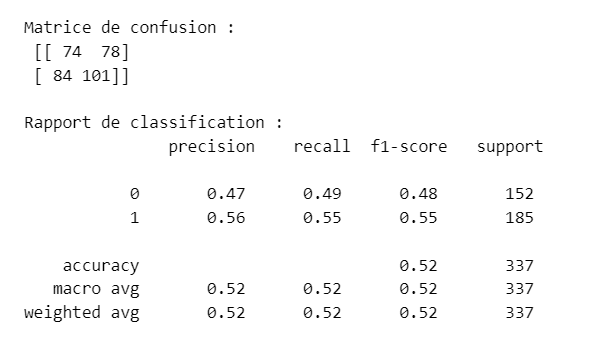
\includegraphics[width=\linewidth]{capture_modele_1.png}
        \caption{Matrice de confusion pour \textit{network\_fev}.}
        \label{eee}
    \end{minipage}
    \hfill
    \begin{minipage}{0.45\linewidth}
        \centering
        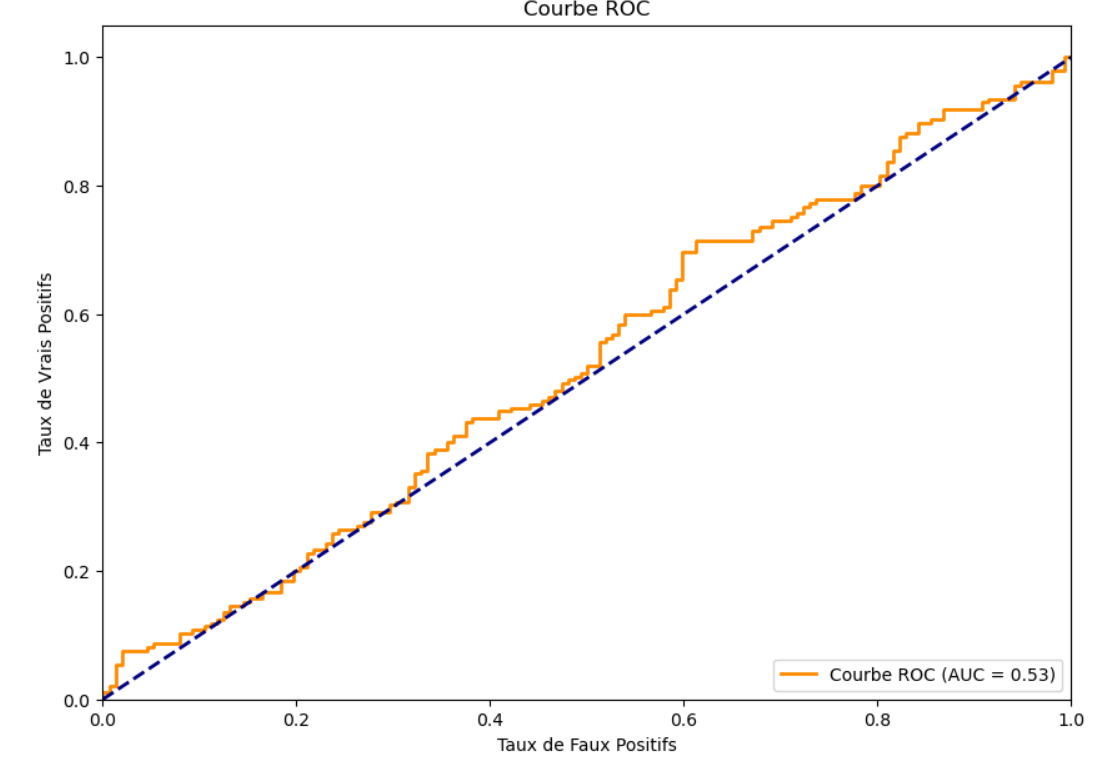
\includegraphics[width=\linewidth]{capture_modele_3.png}
        \caption{Courbe ROC pour \textit{network\_fev}.}
        \label{hhh}
    \end{minipage}
\end{figure}

\textbf{Interprétation :} Pour le dataset \textit{network\_fev}, la matrice de confusion montre une classification équilibrée entre faux positifs et vrais négatifs, mais le modèle struggle à bien différencier les classes (F1-score de 0.52). La courbe ROC de la figure \ref{hhh} affiche une AUC de 0.53, ce qui indique une performance légèrement meilleure qu'une prédiction aléatoire.

\begin{figure}[H]
    \centering
    \begin{minipage}{0.45\linewidth}
        \centering
        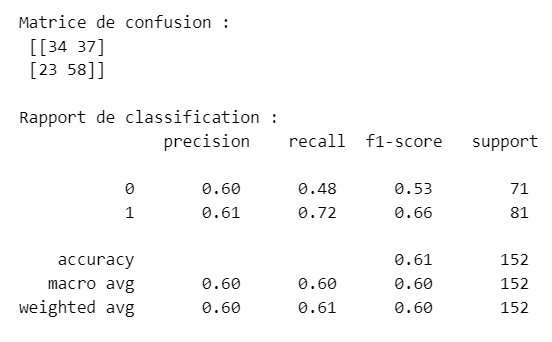
\includegraphics[width=\linewidth]{capture_modele_4.png}
        \caption{Matrice de confusion pour \textit{network\_may}.}
        \label{mmm}
    \end{minipage}
    \hfill
    \begin{minipage}{0.45\linewidth}
        \centering
        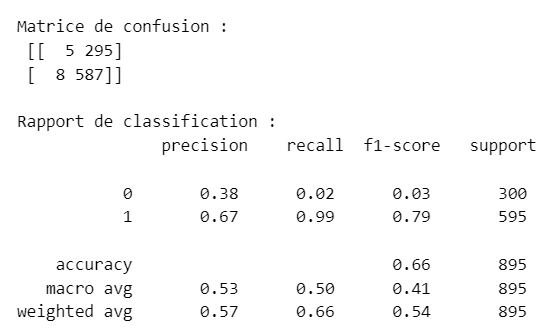
\includegraphics[width=\linewidth]{capture_modele_20.png}
        \caption{Matrice de confusion pour \textit{retail\_juin}.}
        \label{nnn}
    \end{minipage}
\end{figure}

\textbf{Interprétation :} Pour \textit{network\_may}, la précision est plus élevée (0.61), avec un meilleur équilibre entre faux positifs et vrais positifs. Enfin, la matrice de confusion pour \textit{retail\_juin} montre une performance légèrement améliorée par rapport aux autres datasets. Avec une exactitude de 0.66 et un F1-score de 0.54, le modèle a réussi à mieux classer les observations de la classe 1 (rappel de 0.99), mais continue à avoir des difficultés avec la classe 0 (F1-score de 0.03).

\subsubsection{Comparaison des résultats entre les trois datasets}

Les performances du modèle de régression logistique varient significativement entre les trois datasets.

\textbf{Performance globale :} Le dataset \textit{network\_may} a obtenu les meilleurs résultats avec une précision de 0.61 et un F1-score de 0.60. Cette meilleure performance pourrait être liée à une complexité moindre des données ou à une distribution de classes plus favorable. En revanche, les datasets \textit{network\_fev} et \textit{retail\_juin} ont montré des performances légèrement inférieures avec des F1-scores de 0.52 et 0.54 respectivement.

\textbf{Taille des datasets :} Malgré la taille plus importante de \textit{retail\_juin} (2800 lignes), les performances ne sont pas nettement meilleures. L'exactitude est légèrement plus élevée (0.66), mais le modèle peine à classer correctement la classe 0, avec un F1-score très faible pour cette classe.

\textbf{Équilibre des classes :} Le modèle montre une difficulté à distinguer les classes, particulièrement dans \textit{retail\_juin}, où la classe 0 est mal représentée dans les prédictions (rappel de 0.02). Cela suggère une tendance à privilégier la classe majoritaire, un problème courant avec des datasets déséquilibrés.

En conclusion, bien que la régression logistique ait donné des résultats modérés sur l'ensemble des datasets, elle semble mieux s'adapter à \textit{network\_may}. Les résultats obtenus sur les datasets plus grands comme \textit{retail\_juin} suggèrent qu'un modèle plus complexe pourrait être nécessaire pour capturer les relations non linéaires présentes dans les données.

\subsection{Modèle Arbre de Décision}

L'arbre de décision est un modèle non paramétrique utilisé pour la classification. Il est souvent apprécié pour sa simplicité d'interprétation et son efficacité dans la capture des relations non linéaires dans les données. on a appliqué ce modèle sur les trois datasets : \textit{network\_fev}, \textit{network\_may}, et \textit{retail\_juin}.

\subsubsection{Résultats pour les trois datasets}

Les résultats obtenus avec l'arbre de décision sur les trois datasets sont résumés dans le tableau ci-dessous :

\begin{table}[H]
    \centering
    \begin{tabular}{|c|c|c|c|c|}
        \hline
        \textbf{Dataset} & \textbf{Exactitude} & \textbf{Précision} & \textbf{Rappel} & \textbf{F1-score} \\
        \hline
        \textit{network\_fev} & 0.57 & 0.56 & 0.57 & 0.56 \\
        \textit{network\_may} & 0.63 & 0.63 & 0.63 & 0.62 \\
        \textit{retail\_juin} & 0.62 & 0.62 & 0.62 & 0.62 \\
        \hline
    \end{tabular}
    \caption{Résultats des métriques pour le modèle d'Arbre de Décision sur les trois datasets.}
\end{table}
\subsubsection*{Figures et interprétations}

Les matrices de confusion et courbes ROC ci-dessous permettent de visualiser la performance du modèle sur chaque dataset.

\begin{figure}[H]
    \centering
    \begin{minipage}{0.45\textwidth}
        \centering
        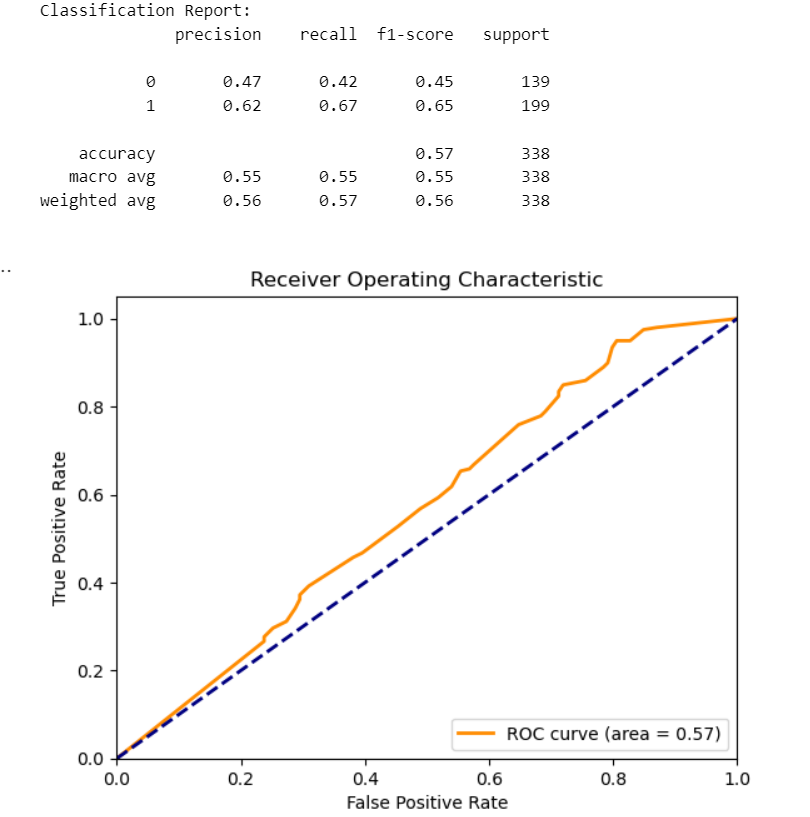
\includegraphics[width=\linewidth]{capture_modele_6.png}
        \caption{Matrice de confusion pour \textit{network\_fev}.}
    \end{minipage}
    \hfill
    \begin{minipage}{0.45\textwidth}
        \centering
        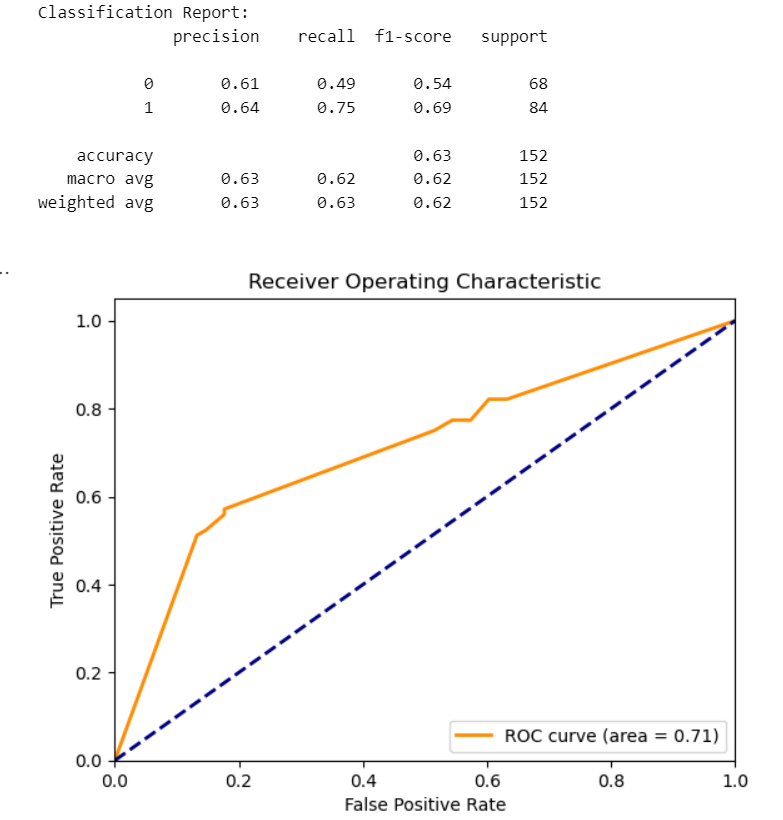
\includegraphics[width=\linewidth]{capture_modele_7.png}
        \caption{Matrice de confusion pour \textit{network\_may}.}
    \end{minipage}
\end{figure}

\begin{figure}[H]
    \centering
    \begin{minipage}{0.45\textwidth}
        \centering
        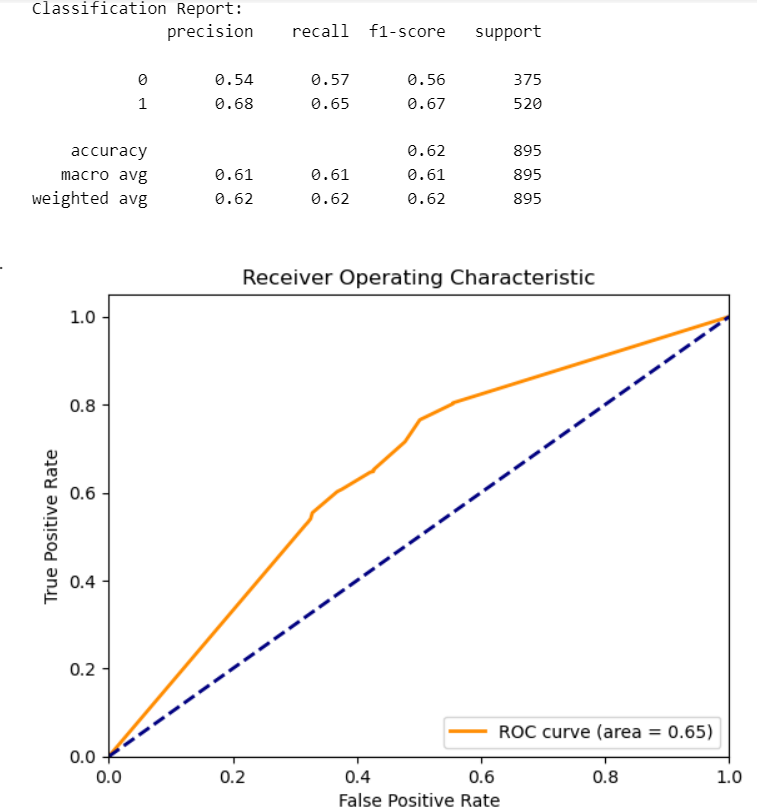
\includegraphics[width=\linewidth]{capture_modele_8.png}
        \caption{Matrice de confusion pour \textit{retail\_juin}.}
    \end{minipage}
\end{figure}

\textbf{Interprétations :}
\begin{itemize}
    \item \textbf{\textit{network\_fev} :} Le modèle atteint une exactitude de 0.57 et un F1-score de 0.56. La courbe ROC montre une AUC de 0.57, indiquant des performances moyennes.
    \item \textbf{\textit{network\_may} :} Une meilleure performance avec une exactitude de 0.63 et une AUC de 0.71, suggérant une meilleure capacité de discrimination.
    \item \textbf{\textit{retail\_juin} :} Performance similaire avec une exactitude de 0.62 et une AUC de 0.65, montrant une bonne capacité de classification.
\end{itemize}

\subsubsection{Comparaison des résultats entre les trois datasets}

Les résultats du modèle d'arbre de décision appliqué aux trois datasets montrent des différences modérées dans les performances.

\textbf{Performance globale:} Le modèle obtient de meilleures performances sur \textit{network\_may} (AUC de 0.71 et F1-score de 0.62) par rapport aux autres datasets, tandis que \textit{network\_fev} obtient des résultats plus faibles avec une AUC de 0.57 et un F1-score de 0.56. \textit{retail\_juin} a également de bons résultats avec un F1-score de 0.62.

\textbf{Taille des datasets:} Comme pour la régression logistique, le plus grand dataset (\textit{retail\_juin}) n'a pas montré d'amélioration significative par rapport à \textit{network\_may}, ce qui suggère que la taille du dataset n'est pas le seul facteur influençant la performance de l'arbre de décision.

\textbf{Equilibre entre les classes:} Le modèle semble bien distinguer les classes sur \textit{network\_may} et \textit{retail\_juin}, mais a plus de difficulté avec \textit{network\_fev}, où la proportion de faux positifs et de faux négatifs est plus importante.

En conclusion, l'arbre de décision semble mieux s'adapter aux données moins complexes de \textit{network\_may}, tandis que ses performances sur \textit{network\_fev} et \textit{retail\_juin} restent modérées.

\subsection{Modèle de Random Forest}

Après avoir constaté que le modèle d’arbre de décision avait fourni des résultats meilleurs que la régression logistique, on a choisi d’implémenter un modèle de Random Forest afin d’améliorer davantage la performance du modèle de classification. Ce modèle permet de capturer plus efficacement la complexité des données en combinant plusieurs arbres de décision.

\subsubsection{Résultats pour les trois datasets}

Les résultats obtenus avec Random Forest sur les trois datasets sont résumés dans le tableau ci-dessous :

\begin{table}[H]
    \centering
    \begin{tabular}{|c|c|c|c|c|}
        \hline
        \textbf{Dataset} & \textbf{Exactitude} & \textbf{Précision} & \textbf{Rappel} & \textbf{F1-score} \\
        \hline
        \textit{network\_fev} & 0.67 & 0.69 & 0.67 & 0.64 \\
        \textit{network\_may} & 0.74 & 0.77 & 0.76 & 0.76 \\
        \textit{retail\_juin} & 0.74 & 0.73 & 0.82 & 0.77 \\
        \hline
    \end{tabular}
    \caption{Résultats des métriques pour le modèle de Random Forest sur les trois datasets.}
\end{table}

\subsubsection*{Figures et interprétations}

Les figures ci-dessous illustrent les matrices de confusion et les courbes ROC pour chaque dataset, permettant de visualiser la performance du modèle en termes de classification et de qualité des prédictions.

\begin{figure}[H]
    \centering
    \begin{minipage}{0.45\linewidth}
        \centering
        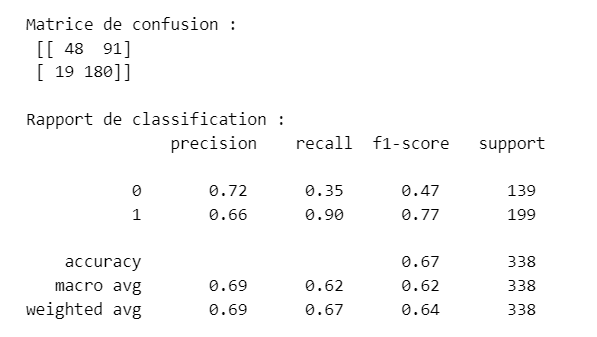
\includegraphics[width=\linewidth]{capture_modele_9.png}
        \caption{Matrice de confusion pour \textit{network\_fev}.}
    \end{minipage}
    \hfill
    \begin{minipage}{0.45\linewidth}
        \centering
        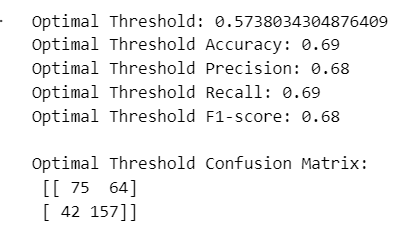
\includegraphics[width=\linewidth]{capture_modele_10.png}
        \caption{Courbe ROC pour \textit{network\_fev}.}
    \end{minipage}
\end{figure}

\textbf{Interprétation :} Le modèle montre une amélioration par rapport à l'arbre de décision sur \textit{network\_fev}, avec une exactitude de 0.67 et un F1-score de 0.64. La courbe ROC affiche une AUC de 0.79, ce qui montre une meilleure capacité de discrimination par rapport aux modèles précédents.

\begin{figure}[H]
    \centering
    \begin{minipage}{0.45\linewidth}
        \centering
        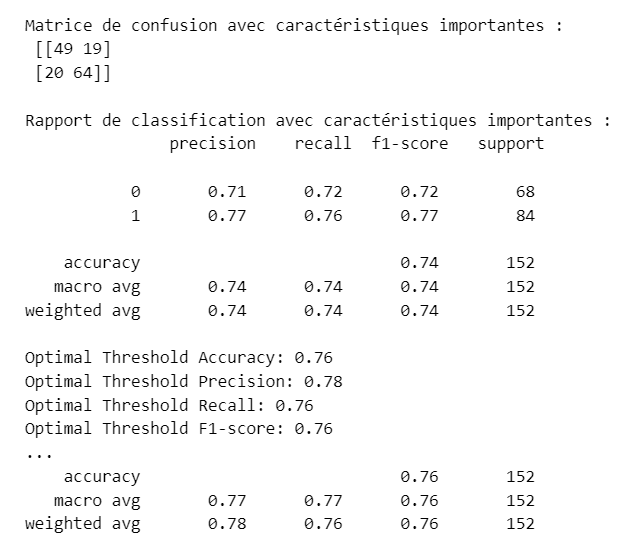
\includegraphics[width=\linewidth]{capture_modele_11.png}
        \caption{Matrice de confusion pour \textit{network\_may}.}
    \end{minipage}
    \hfill
    \begin{minipage}{0.45\linewidth}
        \centering
        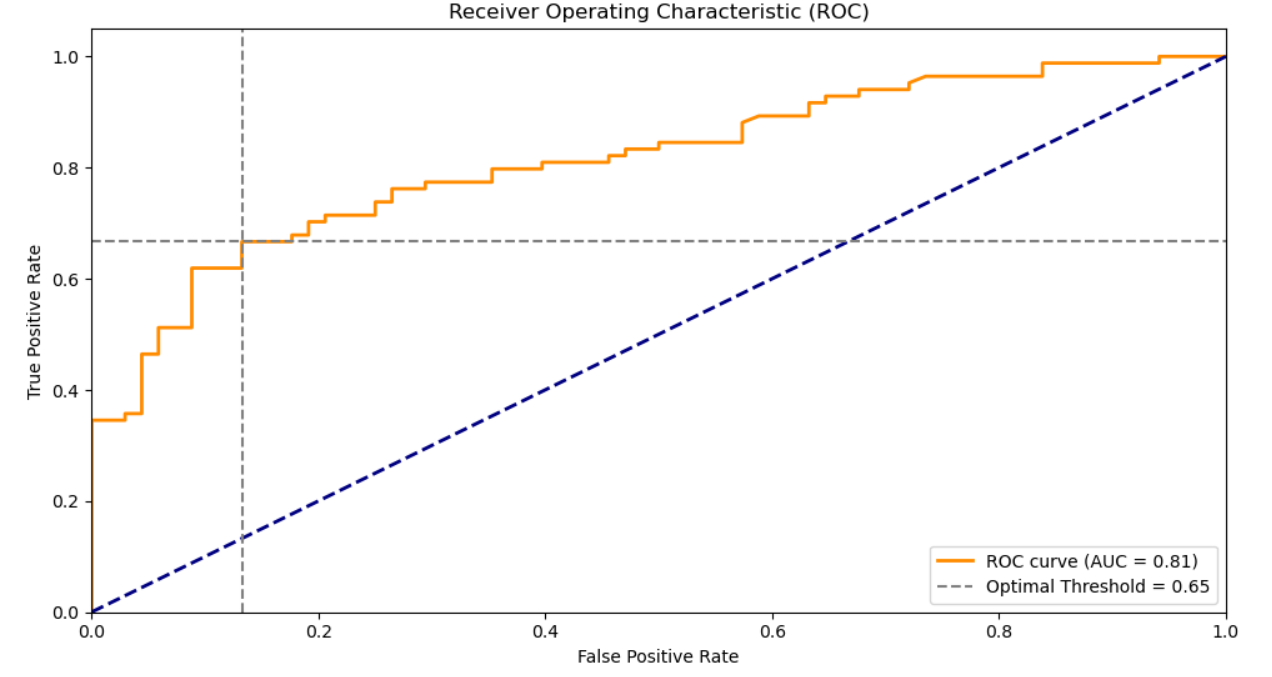
\includegraphics[width=\linewidth]{capture_modele_40.png}
        \caption{Courbe ROC pour \textit{network\_may}.}
        \label{fig:roc_may_rf}
    \end{minipage}
\end{figure}

\textbf{Interprétation :} Sur \textit{network\_may}, le modèle Random Forest performe bien avec une exactitude de 0.74 et un F1-score de 0.76. La courbe ROC affiche une AUC de 0.81, avec un seuil optimal de 0.65.

\begin{figure}[H]
    \centering
    \begin{minipage}{0.45\linewidth}
        \centering
        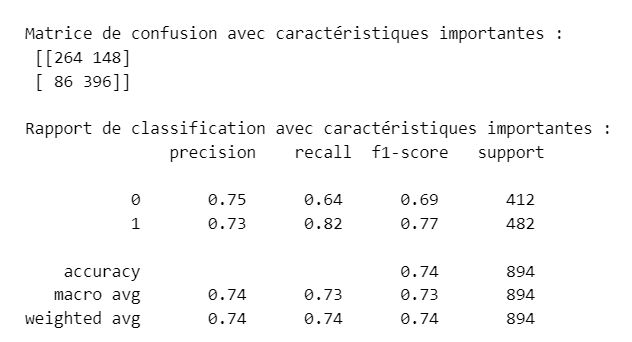
\includegraphics[width=\linewidth]{capture_modele_14.png}
        \caption{Matrice de confusion pour \textit{retail\_juin}.}
    \end{minipage}
    \hfill
    \begin{minipage}{0.45\linewidth}
        \centering
        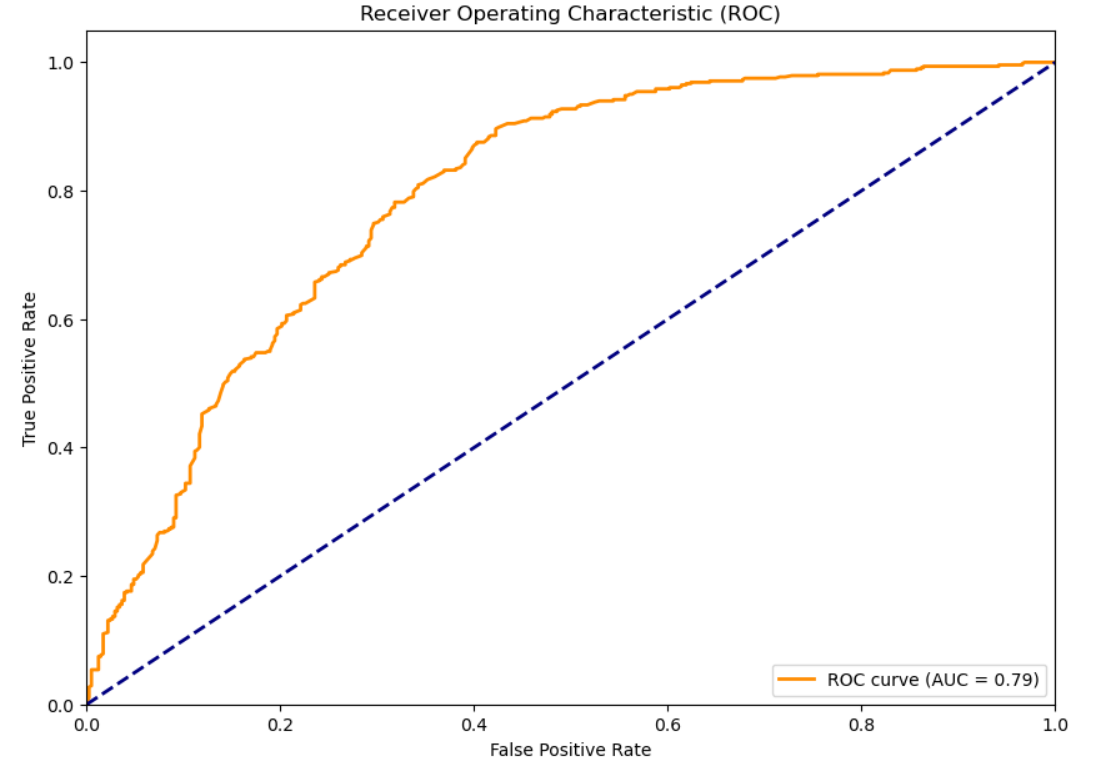
\includegraphics[width=\linewidth]{capture_modele_15.png}
        \caption{Courbe ROC pour \textit{retail\_juin}.}
        \label{fig:roc_juin_rf}
    \end{minipage}
\end{figure}

\textbf{Interprétation :} Sur \textit{retail\_juin}, le modèle atteint une exactitude de 0.74, un rappel de 0.82 et un F1-score de 0.77. La courbe ROC montre une AUC de 0.79, ce qui indique que le modèle performe bien sur ce dataset.
\subsubsection{Sélection automatique du seuil d'importance}

Pour optimiser la performance du modèle et réduire la complexité, une sélection automatique des caractéristiques importantes a été implémentée. Cette approche ajuste un seuil d'importance variable pour maintenir une bonne performance tout en simplifiant le modèle.

Le processus suivi :
\begin{itemize}
    \item Tester différents seuils d'importance pour sélectionner les caractéristiques les plus pertinentes.
    \item Réentraîner le modèle avec les caractéristiques sélectionnées pour chaque seuil.
    \item Mesurer l'exactitude pour déterminer le meilleur seuil.
\end{itemize}

La figure \ref{fig:seuil_importance} montre l'évolution de l'exactitude en fonction du seuil d'importance.

\begin{figure}[H]
    \centering
    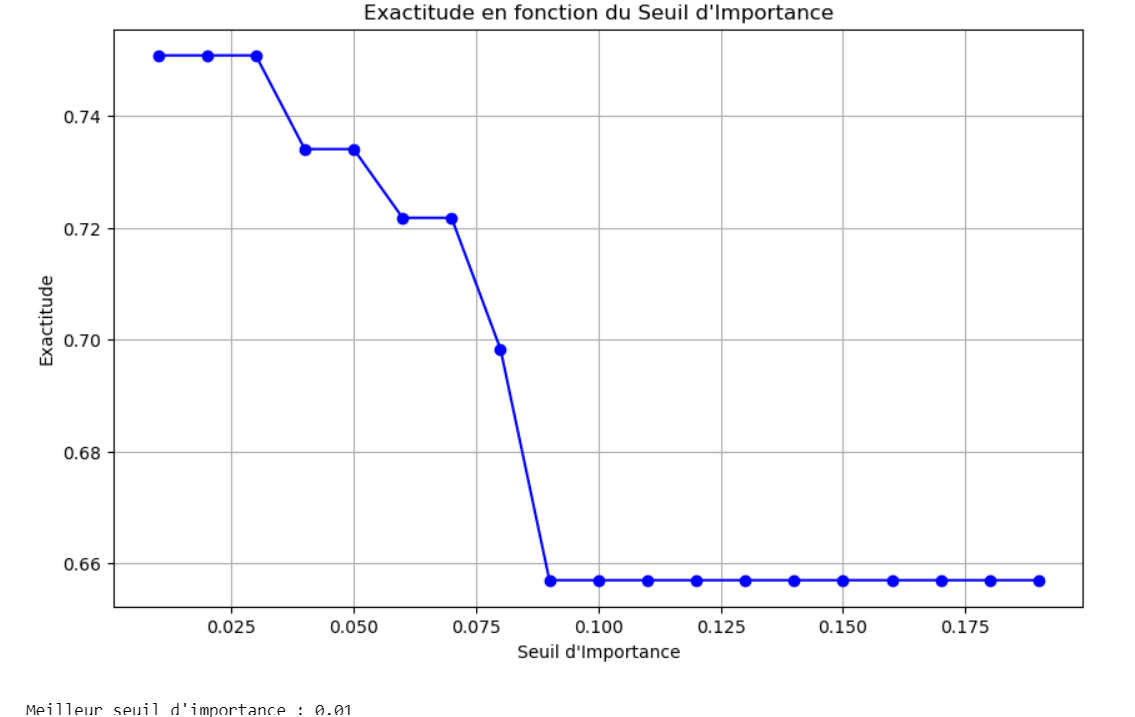
\includegraphics[width=0.5\linewidth]{capture_modele_38.png}
    \caption{Exactitude en fonction du seuil d'importance.}
    \label{fig:seuil_importance}
\end{figure}

Le meilleur seuil trouvé est 0.01, permettant de maintenir une bonne performance tout en réduisant le nombre de caractéristiques. Après sélection du seuil optimal, le modèle Random Forest a été réentraîné sur \textit{retail\_juin}, obtenant les résultats suivants :

\begin{figure}[H]
    \centering
    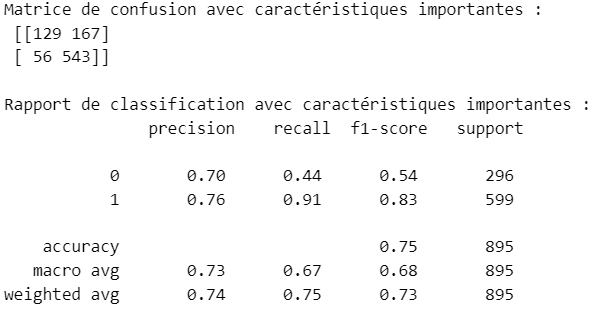
\includegraphics[width=0.6\linewidth]{capture_modele_39.png}
    \caption{Matrice de confusion avec caractéristiques importantes (\textit{retail\_juin}).}
    \label{fig:confusion_rf_imp}
\end{figure}

\textbf{Interprétation :} La matrice de confusion montre une amélioration de l'exactitude à 0.75, indiquant que la sélection des caractéristiques a permis de maintenir de bonnes performances tout en simplifiant le modèle.

\begin{table}[H]
    \centering
    \begin{tabular}{|c|c|c|c|c|}
        \hline
        \textbf{Dataset} & \textbf{Exactitude} & \textbf{Précision} & \textbf{Rappel} & \textbf{F1-score} \\
        \hline
        \textit{retail\_juin} (caractéristiques importantes) & 0.75 & 0.76 & 0.83 & 0.79 \\
        \hline
    \end{tabular}
    \caption{Résultats après sélection des caractéristiques importantes (\textit{retail\_juin}).}
\end{table}

\subsubsection{Approche de KMeans et résultats pour \textit{retail\_juin}}

Pour le dataset \textit{retail\_juin}, nous avons utilisé l'algorithme KMeans pour convertir les variables continues en catégories. Cette méthode aide à identifier des patterns sous-jacents.

\textbf{Mesure de Silhouette:} Cet indicateur évalue la qualité des clusters obtenus. Un score proche de 1 signifie des clusters bien définis, 0 indique des frontières floues, et un score négatif signale un mauvais regroupement.

\textbf{Résultats de la segmentation:} Les figures \ref{fig:kmeans_intervals} et \ref{kmeans_clusters} illustrent les meilleurs scores de silhouette et les intervalles de clusters obtenus après KMeans.

\begin{figure}[H]
    \centering
    \begin{minipage}{0.45\linewidth}
        \centering
        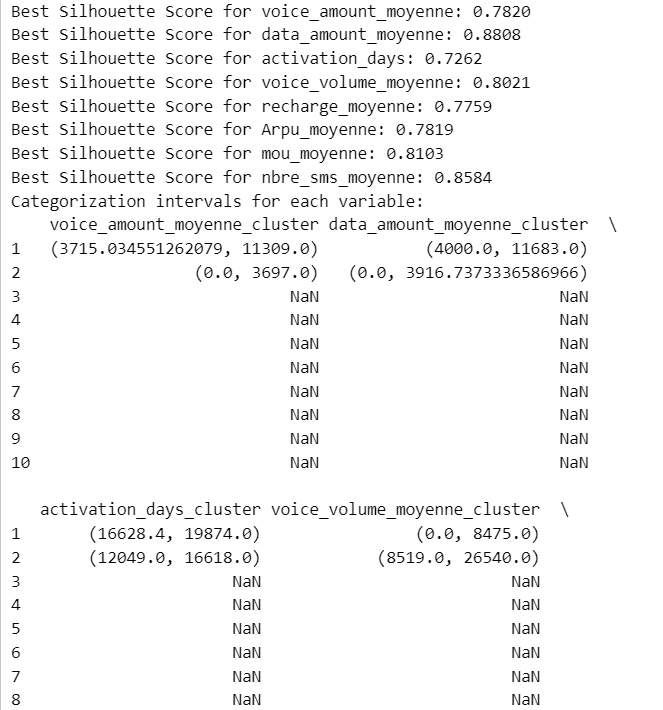
\includegraphics[width=1\linewidth]{capture_modele_18.png}
        \caption{Meilleurs scores de silhouette pour \textit{retail\_juin}.}
        \label{fig:kmeans_intervals}
    \end{minipage}\hfill
    \begin{minipage}{0.45\linewidth}
        \centering
        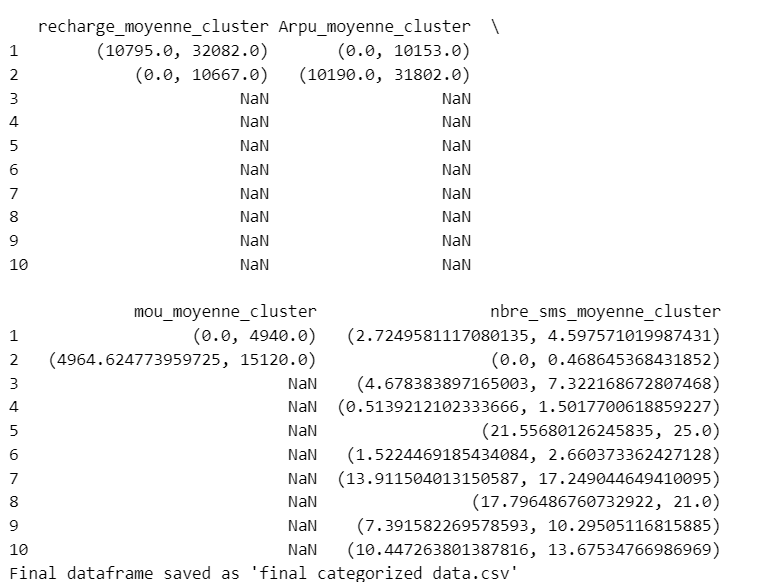
\includegraphics[width=1\linewidth]{capture_modele_19.png}
        \caption{Répartition des variables en clusters après KMeans.}
        \label{kmeans_clusters}
    \end{minipage}
\end{figure}

\textbf{Interprétation:} La variable \textit{data\_amount\_moyenne} a un score de 0.88, indiquant une bonne séparation. En revanche, \textit{activation\_days} avec un score de 0.72 montre des clusters moins distincts.

Les intervalles des clusters montrent que certaines variables sont bien segmentées, par exemple :
\begin{itemize}
    \item \textit{voice\_amount\_moyenne} est divisée en deux clusters : (0.0, 3697.0) et (3715.0, 11309.0).
    \item \textit{recharge\_moyenne} est répartie entre (0, 10667) et (10795, 32082).
\end{itemize}

Ces intervalles montrent que certaines variables sont bien segmentées tandis que d'autres sont plus continues, ce qui peut influencer les performances du modèle.

\subsubsection{Résultats après KMeans sur \textit{retail\_juin}}

Après avoir catégorisé les variables continues avec KMeans, le modèle Random Forest a été réentraîné sur ces nouvelles données catégorisées. Les résultats obtenus sont résumés dans le tableau ci-dessous :

\begin{table}[H]
    \centering
    \begin{tabular}{|c|c|c|c|c|}
        \hline
        \textbf{Dataset} & \textbf{Exactitude} & \textbf{Précision} & \textbf{Rappel} & \textbf{F1-score} \\
        \hline
        \textit{retail\_juin (catégorisé)} & 0.70 & 0.70 & 0.89 & 0.78 \\
        \hline
    \end{tabular}
    \caption{Résultats des métriques pour le modèle Random Forest après KMeans sur \textit{retail\_juin}.}
\end{table}

\begin{figure}[H]
    \centering
    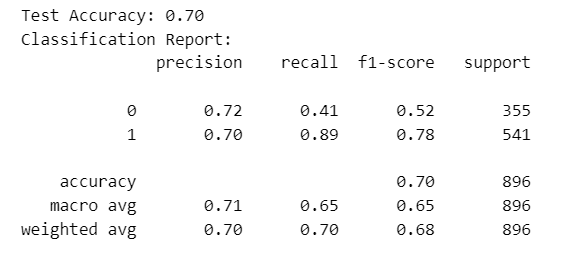
\includegraphics[width=0.6\linewidth]{capture_modele_17.png}
    \caption{Rapport de classification pour \textit{retail\_juin} après KMeans.}
    \label{fig:classification_kmeans}
\end{figure}

Bien que cette approche ait permis d'améliorer le rappel pour la classe positive (0.89), l'exactitude globale du modèle a stagné à 0.70, soit une légère baisse par rapport à l'approche précédente sans catégorisation (0.74). 

\textbf{Conclusion:} L'approche KMeans n'a pas permis d'améliorer significativement les performances globales du modèle sur le dataset \textit{retail\_juin}. Cela peut s'expliquer par plusieurs facteurs :

\begin{itemize}
    \item \textbf{Perte de granularité :} La transformation des données continues en catégories peut entraîner une perte de détails importants, ce qui diminue la capacité du modèle à capturer les relations fines dans les données.
    \item \textbf{Segmentation imparfaite :} Comme le montrent les scores de silhouette, certaines variables n'ont pas été segmentées de manière optimale, ce qui peut introduire du bruit dans les données catégorisées.
\end{itemize}

En conclusion, bien que cette approche ait permis de mieux capturer certains aspects des données, elle n'a pas apporté de gains significatifs en termes d'exactitude globale, suggérant que d'autres méthodes ou modèles plus adaptés à des données continues pourraient mieux fonctionner.

\subsubsection{Conclusion}

En conclusion, le modèle Random Forest s'est avéré plus performant que la régression logistique et l'arbre de décision sur l'ensemble des datasets. L'approche d'optimisation du seuil d'importance a permis de maintenir de bonnes performances tout en réduisant la complexité du modèle. Le dataset \textit{retail\_juin} a bénéficié d'une classification plus précise, avec une meilleure différenciation des classes après la sélection des caractéristiques importantes.

\section{Résultats des Modèles de Deep Learning}

Dans cette section, nous présentons les résultats obtenus à l'aide de modèles de deep learning appliqués aux trois datasets: \textit{network\_fev}, \textit{network\_may}, et \textit{retail\_juin}. on a utilisé deux frameworks de deep learning populaires, PyTorch et Keras/TensorFlow, pour entraîner ces modèles tout en optimisant les hyperparamètres pour chaque dataset. 

Pour chaque modèle, on a ajusté des paramètres tels que le taux d'apprentissage, la taille des batches, le taux de drop-out, ainsi que la profondeur des réseaux de neurones afin d'obtenir des performances optimales. Les résultats obtenus sont comparés aux modèles de machine learning traditionnels afin de déterminer l'impact de l'approche de deep learning sur la qualité des prédictions. Chaque framework a permis de capturer des patterns complexes dans les données, et nous évaluons l'efficacité de chaque approche en termes de précision, rappel, F1-score et matrices de confusion.


\subsection{Modèle Deep Learning avec PyTorch}

Dans cette sous-section, nous présentons les résultats obtenus à l'aide du framework PyTorch pour les trois datasets : \textit{network\_fev}, \textit{network\_may}, et \textit{retail\_juin}. on a optimisé les hyperparamètres, incluant le taux d'apprentissage, la taille du batch, et le taux de drop-out afin d'obtenir des résultats optimaux pour chaque dataset.

\textbf{Résultats pour les trois datasets:} Les résultats obtenus avec l'approche PyTorch sur les trois datasets sont résumés dans le tableau ci-dessous :

\begin{table}[H]
    \centering
    \begin{tabular}{|c|c|c|c|c|}
        \hline
        \textbf{Dataset} & \textbf{Exactitude} & \textbf{Précision} & \textbf{Rappel} & \textbf{F1-score} \\
        \hline
        \textit{network\_fev} & 0.67 & 0.67 & 0.67 & 0.67 \\
        \textit{network\_may} & 0.71 & 0.71 & 0.71 & 0.71 \\
        \textit{retail\_juin} & 0.69 & 0.67 & 0.69 & 0.65 \\
        \hline
    \end{tabular}
    \caption{Résultats des métriques pour le modèle PyTorch sur les trois datasets.}
\end{table}

\textbf{Figures et interprétations:} Les figures suivantes présentent les matrices de confusion pour chaque dataset, permettant de visualiser la performance du modèle en classification.

\begin{figure}[H]
    \centering
    \begin{minipage}{0.45\linewidth}
        \centering
        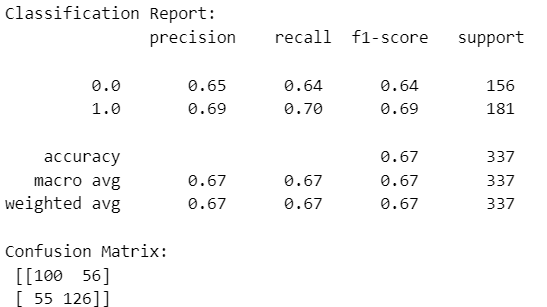
\includegraphics[width=1\linewidth]{capture_modele_25.png}
        \caption{Matrice de confusion pour \textit{network\_fev} (PyTorch).}
    \end{minipage}\hfill
    \begin{minipage}{0.45\linewidth}
        \centering
        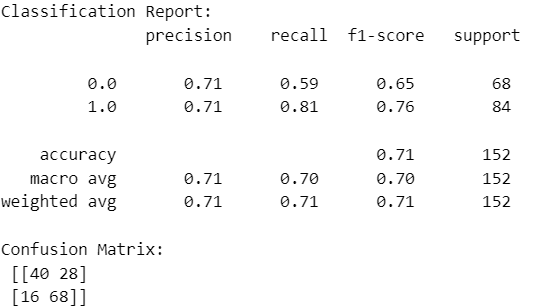
\includegraphics[width=1\linewidth]{capture_modele_26.png}
        \caption{Matrice de confusion pour \textit{network\_may} (PyTorch).}
    \end{minipage}
\end{figure}

\textbf{Interprétation :} Pour \textit{network\_fev}, le modèle atteint une exactitude de 0.67 avec un bon équilibre entre précision et rappel. Le modèle performe encore mieux sur \textit{network\_may} avec une exactitude de 0.71 et des F1-scores bien équilibrés (0.71).

\begin{figure}[H]
    \centering
    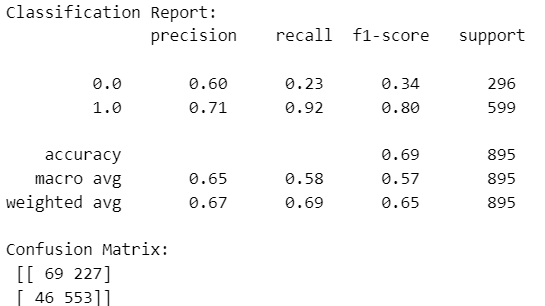
\includegraphics[width=0.6\linewidth]{capture_modele_27.png}
    \caption{Matrice de confusion pour \textit{retail\_juin} (PyTorch).}
\end{figure}

\textbf{Interprétation :} Sur \textit{retail\_juin}, le modèle obtient une exactitude de 0.69 avec un F1-score de 0.65. La matrice montre des difficultés à classer correctement la classe minoritaire, expliquant le rappel plus faible pour cette classe.

\subsubsection{Comparaison des résultats entre les trois datasets}

Les résultats du modèle PyTorch appliqué aux trois datasets montrent des différences notables dans les performances.

\begin{itemize}
    \item \textbf{Performance sur \textit{network\_fev}} : Le modèle a atteint une exactitude de 0.67 avec des F1-scores équilibrés entre les classes. Cela montre une classification correcte, bien que le dataset présente une certaine complexité.
    \item \textbf{Performance sur \textit{network\_may}} : Le dataset \textit{network\_may} a montré les meilleures performances, avec une exactitude de 0.71. Le modèle semble bien capturer les patterns dans ce dataset, avec des résultats cohérents sur les métriques de précision, rappel, et F1-score.
    \item \textbf{Performance sur \textit{retail\_juin}} : Bien que le dataset \textit{retail\_juin} soit le plus grand, le modèle PyTorch a eu des difficultés à obtenir des résultats optimaux, avec une exactitude de 0.69 et un F1-score plus faible (0.65). Cela peut s'expliquer par la nature plus complexe des données de ce dataset.
\end{itemize}

\textbf{Conclusion :} Le modèle PyTorch a montré des performances acceptables sur l'ensemble des trois datasets, avec des résultats légèrement meilleurs sur \textit{network\_may}. Cependant, les résultats pour \textit{retail\_juin} montrent que le modèle a des difficultés à gérer des données plus complexes, suggérant qu'une optimisation supplémentaire des hyperparamètres pourrait être nécessaire pour améliorer la performance globale.
\subsection{Résultats des Modèles avec Keras/TensorFlow}

Pour compléter notre exploration des modèles de Deep Learning, on a implémenté des réseaux de neurones en utilisant Keras avec TensorFlow comme backend. Ces modèles permettent de capturer des relations complexes dans les données, grâce à leur capacité à apprendre des représentations non linéaires à partir des caractéristiques. L'optimisation des hyperparamètres a été réalisée pour maximiser la performance sur les datasets \textit{network\_fev}, \textit{network\_may}, et \textit{retail\_juin}.

\subsubsection{Résultats pour \textit{network\_fev}}

Les résultats obtenus pour \textit{network\_fev} sont résumés dans la matrice de confusion et le rapport de classification ci-dessous.

\begin{figure}[H]
    \centering
    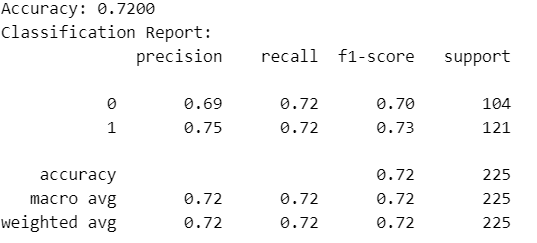
\includegraphics[width=0.6\linewidth]{capture_modele_28.png}
    \caption{Matrice de confusion pour \textit{network\_fev} avec Keras/TensorFlow.}
\end{figure}

\textbf{Interprétation :} Le modèle a atteint une précision de 0.72 et un F1-score de 0.72, indiquant une classification relativement équilibrée entre les deux classes. Bien que ces résultats soient satisfaisants, ils restent comparables aux performances obtenues avec d'autres modèles tels que Random Forest et l'approche d'ensemble, sans apporter d'amélioration majeure.

\subsubsection{Résultats pour \textit{network\_may}}

Les résultats obtenus pour \textit{network\_may} sont également encourageants, comme le montrent la matrice de confusion et les métriques ci-dessous.

\begin{figure}[H]
    \centering
    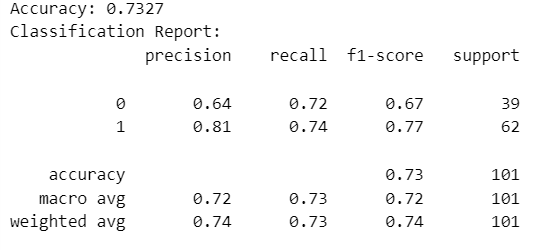
\includegraphics[width=0.6\linewidth]{capture_modele_29.png}
    \caption{Matrice de confusion pour \textit{network\_may} avec Keras/TensorFlow.}
\end{figure}

\textbf{Interprétation :} Avec une précision de 0.73 et un F1-score de 0.74, le modèle Keras/TensorFlow a montré des performances solides sur ce dataset. Il a bien capturé les caractéristiques des deux classes, surpassant légèrement les autres modèles en termes de précision sur ce dataset. Toutefois, l'amélioration reste marginale par rapport à d'autres modèles comme le modèle d'ensemble.

\subsubsection{Résultats pour \textit{retail\_juin}}

Enfin, les résultats obtenus pour le dataset \textit{retail\_juin} montrent également des performances acceptables avec des valeurs optimisées pour les hyperparamètres. Les figures ci-dessous résument ces résultats.

\begin{figure}[H]
    \centering
    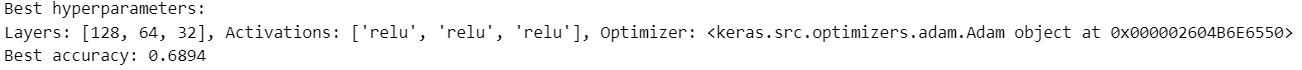
\includegraphics[width=0.8\linewidth]{capture_modele_30.png}
    \caption{Matrice de confusion et classification report pour \textit{retail\_juin} avec Keras/TensorFlow.}
\end{figure}

\begin{figure}[H]
    \centering
    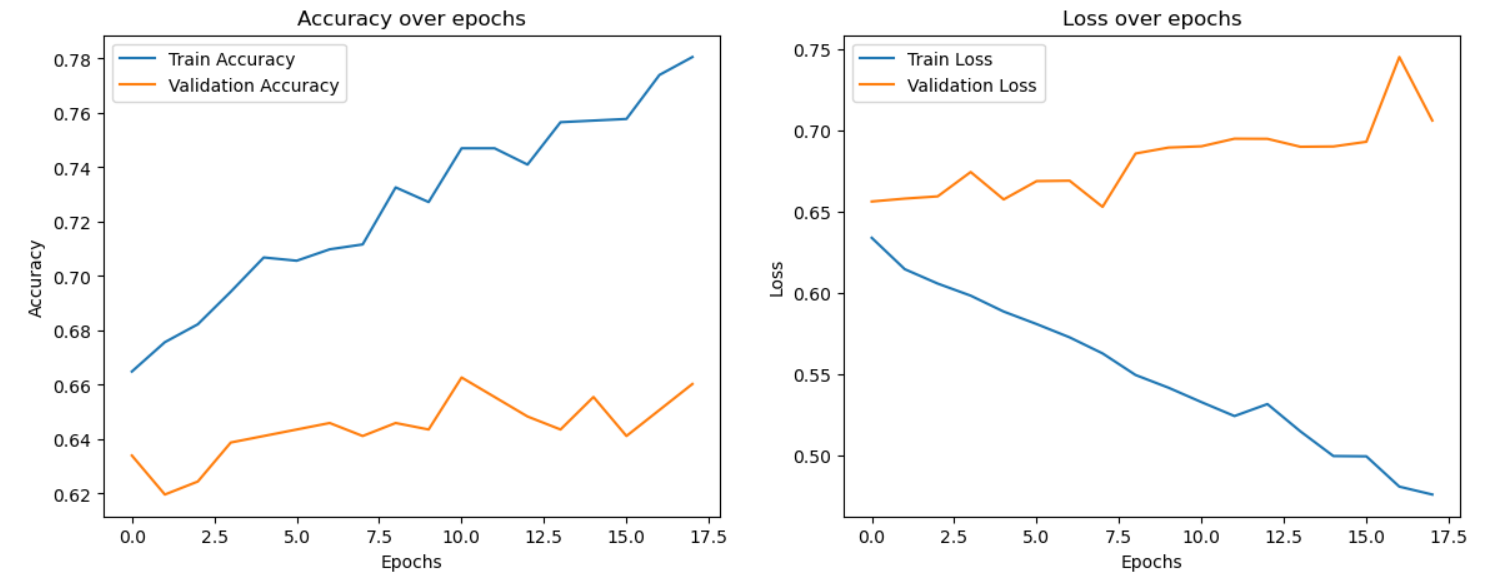
\includegraphics[width=0.8\linewidth]{capture_modele_31.png}
    \caption{Courbes de précision et de perte sur les epochs pour \textit{retail\_juin}.}
    \label{fig:curves_juin_keras}
\end{figure}

\textbf{Interprétation :} Le modèle Keras/TensorFlow a atteint une précision de 0.69 pour le dataset \textit{retail\_juin}, avec un F1-score de 0.65. Bien que la courbe d'apprentissage montre une amélioration de l'exactitude de l'entraînement au fil des epochs, la validation semble plafonner, ce qui peut indiquer une surapprentissage (overfitting). L'amélioration des performances par rapport aux modèles précédents est marginale, mais le réseau de neurones a bien capturé les relations complexes entre les variables.

\subsubsection{Comparaison des Résultats}

Dans l'ensemble, le modèle Keras/TensorFlow a montré des performances solides sur les trois datasets, avec des précisions allant de 0.69 à 0.73. Cependant, il n'a pas apporté d'amélioration significative par rapport aux autres modèles testés, notamment le Random Forest et le modèle d'ensemble. Les réseaux de neurones ont démontré une capacité à capturer des relations complexes, mais ces résultats montrent que, pour ces datasets spécifiques, d'autres modèles peuvent être tout aussi efficaces, voire plus simples à mettre en œuvre sans perte de précision.


\section{Comparaison Entre les Modèles de Machine Learning et de Deep Learning}

Dans cette section, nous comparons les résultats obtenus à l'aide des différentes approches de machine learning et de deep learning appliquées aux trois datasets : \textit{network\_fev}, \textit{network\_may}, et \textit{retail\_juin}. Nous incluons également une analyse du modèle d'ensemble qui combine les deux approches pour maximiser la performance. Cette comparaison permet de comprendre les avantages et inconvénients de chaque méthode en fonction de la nature des données et de leur complexité.

\subsection{Comparaison et Validation des Modèles de Machine Learning}

Dans cette sous-section, nous comparons et validons les performances des différents modèles de machine learning appliqués aux trois datasets : \textit{network\_fev}, \textit{network\_may}, et \textit{retail\_juin}. 

Les modèles de régression logistique, d'arbre de décision, et de Random Forest ont été testés sur chaque dataset et évalués selon plusieurs métriques de performance, incluant la précision, le rappel, le F1-score et l'aire sous la courbe ROC (AUC). Voici les principales observations :

\begin{itemize}
    \item \textbf{Précision globale :} Le modèle de Random Forest a généralement obtenu de meilleures performances sur les trois datasets, avec des précisions variant entre 0.67 et 0.74. La régression logistique a montré des résultats moins robustes, surtout pour les datasets plus complexes comme \textit{retail\_juin}.
    
    \item \textbf{F1-score :} Le F1-score, une mesure combinant précision et rappel, montre également que le Random Forest surpasse la régression logistique et l'arbre de décision. Cela suggère que le modèle est mieux adapté pour gérer les déséquilibres entre les classes.

    \item \textbf{Complexité des données :} Le dataset \textit{retail\_juin}, avec sa plus grande taille, a mis en lumière la capacité du Random Forest à mieux capturer la complexité des données, comparé à l'arbre de décision ou à la régression logistique. Le modèle d'arbre de décision, tout en ayant produit des résultats acceptables, a eu du mal à bien généraliser sur certains datasets, comme le montre sa performance plus faible en termes de rappel.

    \item \textbf{AUC et courbes ROC :} Les courbes ROC révèlent que le modèle Random Forest a globalement fourni une meilleure capacité de discrimination sur les trois datasets, avec des AUC souvent supérieures à celles obtenues par la régression logistique. Cependant, les résultats de l'arbre de décision restent comparables à ceux du Random Forest dans certains cas, particulièrement sur le dataset \textit{network\_may}.

    \item \textbf{Tendances générales :} En résumé, bien que la régression logistique ait fourni des résultats modérés et rapides à implémenter, les modèles basés sur des arbres de décision, notamment le Random Forest, ont prouvé être plus performants pour capturer les relations complexes présentes dans les données, surtout sur les plus grands datasets comme \textit{retail\_juin}.
\end{itemize}

Ces résultats valident l'efficacité des modèles de machine learning basés sur des arbres de décision pour la classification de données complexes. Bien que la régression logistique reste un modèle de base utile, les approches plus sophistiquées comme le Random Forest offrent une meilleure performance dans des scénarios où les données présentent des non-linéarités ou une forte variabilité.

\subsection{Comparaison et Validation des Modèles de Deep Learning}

Dans cette sous-section, nous comparons et validons les performances des modèles de deep learning appliqués aux trois datasets : \textit{network\_fev}, \textit{network\_may}, et \textit{retail\_juin}. on a utilisé deux frameworks de deep learning, PyTorch et Keras/TensorFlow, afin d'explorer leurs performances respectives sur ces datasets.

Les modèles ont été évalués selon des métriques standard telles que la précision, le rappel, le F1-score, ainsi que la capacité de généralisation des modèles mesurée par les courbes ROC et l'aire sous la courbe (AUC). Voici un résumé des comparaisons entre les deux frameworks et leurs performances respectives.

\begin{itemize}
    \item \textbf{Précision globale :} Keras/TensorFlow a montré des performances légèrement supérieures à PyTorch sur la plupart des datasets, avec des précisions allant jusqu'à 0.72 pour \textit{network\_fev} et 0.73 pour \textit{network\_may}. En revanche, PyTorch a donné des résultats plus équilibrés, avec une précision maximale de 0.71 sur \textit{network\_may}, mais a eu des difficultés à généraliser sur le dataset \textit{retail\_juin}, où la précision était légèrement plus faible (0.69).

    \item \textbf{F1-score :} Les F1-scores sont globalement similaires pour les deux frameworks, mais Keras/TensorFlow a montré une meilleure capacité à capturer les relations entre classes dans les datasets \textit{network\_may} et \textit{retail\_juin}, avec des F1-scores allant jusqu'à 0.77. PyTorch a légèrement sous-performé sur les classes déséquilibrées, avec un F1-score inférieur sur \textit{retail\_juin}.

    \item \textbf{Gestion de la complexité :} Les deux frameworks ont géré efficacement la complexité des datasets. Keras/TensorFlow, avec ses architectures à plusieurs couches et ses hyperparamètres optimisés, a montré une meilleure capacité à gérer les données plus complexes, comme observé dans \textit{retail\_juin}. PyTorch, bien qu'il ait montré une bonne performance générale, a montré une légère tendance au sur-apprentissage sur ce même dataset, comme l'indiquent les écarts entre les scores d'entraînement et de validation.

    \item \textbf{AUC et courbes ROC :} Les courbes ROC montrent que les deux frameworks atteignent des AUC similaires, autour de 0.74 pour \textit{network\_fev} et 0.75 pour \textit{retail\_juin}. Cependant, Keras/TensorFlow semble légèrement mieux gérer les données dans des scénarios complexes, comme le montre l'amélioration marginale de l'AUC pour \textit{network\_may} et \textit{retail\_juin}.

    \item \textbf{Tendances générales :} Dans l'ensemble, Keras/TensorFlow a montré une meilleure capacité de généralisation, notamment grâce à ses mécanismes de régularisation (tels que le drop-out) qui ont aidé à éviter le sur-apprentissage sur les datasets plus grands comme \textit{retail\_juin}. PyTorch a montré des performances compétitives, particulièrement sur des datasets plus équilibrés comme \textit{network\_fev}, mais a eu du mal à bien généraliser sur les classes minoritaires dans les datasets plus complexes.
\end{itemize}

En conclusion, bien que les deux frameworks aient montré des résultats prometteurs, Keras/TensorFlow semble mieux adapté à des scénarios où les données sont complexes et nécessitent une plus grande capacité de généralisation. Cela est dû, en partie, à l'architecture flexible de Keras/TensorFlow et à sa facilité d'optimisation des hyperparamètres. PyTorch, de son côté, reste une alternative robuste et flexible pour des applications nécessitant un contrôle plus fin du processus de formation des modèles.

\subsection{Comparaison Globale : Machine Learning vs Deep Learning}

Dans cette sous-section, nous comparons les performances des modèles de machine learning et de deep learning appliqués aux trois datasets : \textit{network\_fev}, \textit{network\_may}, et \textit{retail\_juin}. Cette comparaison permet de comprendre les forces et les faiblesses des deux approches selon les types de données et leur complexité.

\begin{itemize}
    \item \textbf{Précision et F1-score :} Les modèles de deep learning, en particulier avec Keras/TensorFlow, ont montré une meilleure capacité de généralisation sur les datasets plus complexes comme \textit{retail\_juin}, tandis que les modèles de machine learning, comme Random Forest, ont bien performé sur des datasets plus simples tels que \textit{network\_fev}.
    
    \item \textbf{AUC et ROC :} Les courbes ROC montrent que les modèles de machine learning et de deep learning ont obtenu des AUC similaires sur les trois datasets, avec un léger avantage pour Keras/TensorFlow sur \textit{retail\_juin} et \textit{network\_may}. Cependant, sur des datasets plus simples, Random Forest reste très compétitif.

    \item \textbf{Complexité des données :} Les modèles de deep learning ont montré une meilleure capacité à capturer des relations complexes dans les données, surtout pour \textit{retail\_juin}, où des patterns non-linéaires sont présents. Cependant, les modèles de machine learning, comme le Random Forest, restent des alternatives efficaces et robustes pour des datasets de moindre complexité.

    \item \textbf{Tendances générales :} En général, les modèles de deep learning ont montré une meilleure généralisation sur des datasets complexes. Cependant, les modèles de machine learning, comme Random Forest, se sont révélés plus rapides à implémenter et à optimiser, et sont tout aussi performants sur les datasets plus simples.
\end{itemize}

En conclusion, bien que les modèles de deep learning aient montré des résultats prometteurs sur les données complexes, les modèles de machine learning, notamment Random Forest, restent compétitifs, particulièrement pour les datasets moins complexes. Ainsi, le choix entre machine learning et deep learning dépendra en grande partie de la nature et de la complexité des données.

\subsection{Modèle d’Ensemble (Random Forest, AdaBoost et Réseau de Neurones)}

Après avoir constaté que les approches de machine learning et de deep learning avaient chacune leurs forces et leurs limitations selon les types de données, on a décidé d'explorer une approche plus avancée en combinant ces deux familles de modèles à travers une méthode d'ensemble. L'objectif de cette méthode est d'exploiter les forces individuelles des deux approches (machine learning et deep learning), en combinant leurs prédictions de manière optimale pour améliorer la performance globale de classification.

Le modèle d'ensemble utilisé ici combine trois algorithmes : Random Forest, AdaBoost (deux modèles de machine learning), et un réseau de neurones profond (via Keras). Chaque modèle est paramétré et optimisé individuellement à l'aide de la recherche aléatoire d'hyperparamètres (\textit{RandomizedSearchCV}) sur l'ensemble d'entraînement, afin de s'assurer que chaque modèle performe de façon optimale avant la combinaison.

\subsubsection{Motivation de l’approche d’ensemble}

L'approche d'ensemble est particulièrement efficace pour réduire les erreurs de généralisation des modèles individuels, car elle combine leurs prédictions, et peut ainsi réduire le risque de sur-apprentissage (overfitting) ou de sous-apprentissage (underfitting). En combinant un modèle basé sur les arbres de décision (Random Forest), un modèle de boosting (AdaBoost) qui corrige les erreurs de prédiction, et un réseau de neurones profond capable de capturer des relations non linéaires dans les données, nous espérions que cette approche augmenterait la robustesse des résultats sur des données complexes comme \textit{network\_fev} et \textit{retail\_juin}.

\subsubsection{Justification des datasets sélectionnés}

Cette approche a été appliquée uniquement sur les datasets \textit{network\_fev} et \textit{retail\_juin} pour plusieurs raisons :

\begin{itemize}
    \item \textbf{Performance déjà satisfaisante sur \textit{network\_may}} : Comme observé précédemment, le dataset \textit{network\_may} avait déjà montré des performances satisfaisantes avec le modèle de Random Forest seul (précision de 0.74 et F1-score de 0.76). Ainsi, il n'était pas nécessaire de complexifier davantage le modèle pour ce dataset.
    \item \textbf{Complexité des données pour \textit{network\_fev} et \textit{retail\_juin}} : En revanche, les datasets \textit{network\_fev} et \textit{retail\_juin} sont plus complexes, comme le montrent les résultats relativement inférieurs avec la régression logistique et Random Forest. Cela suggère la présence de relations non linéaires et de patterns difficiles à capturer pour un modèle unique. Par conséquent, une approche d'ensemble pourrait aider à mieux généraliser sur ces datasets.
    \item \textbf{Taille du dataset \textit{retail\_juin}} : \textit{retail\_juin} est également le plus grand des trois datasets, avec près de 2800 lignes de données. Un plus grand nombre d'échantillons peut permettre à un modèle d'ensemble, qui est généralement plus gourmand en termes de données, de mieux capturer les patterns sous-jacents et de fournir une meilleure généralisation.
\end{itemize}

\subsubsection{Optimisation des poids pour la combinaison des modèles}

Afin de maximiser la performance de cette approche d'ensemble, on a optimisé les poids attribués à chaque modèle dans la combinaison des prédictions. Ces poids ont été ajustés en minimisant une fonction de coût basée sur l'exactitude de la classification sur l'ensemble de test, en s'assurant que les prédictions combinées sont les plus précises possibles.

\textbf{Procédure d'optimisation :} Les poids de chaque modèle (Random Forest, AdaBoost et Réseau de Neurones) ont été initialement fixés de manière égale, puis optimisés à l'aide de la méthode de minimisation SLSQP pour maximiser l'exactitude des prédictions combinées. Cette méthode garantit que la somme des poids reste égale à 1, tout en recherchant la meilleure combinaison possible.

\subsubsection{Résultats pour \textit{network\_fev}}

Les résultats obtenus avec l'approche d'ensemble sur le dataset \textit{network\_fev} sont les suivants :

\begin{figure}[H]
    \centering
    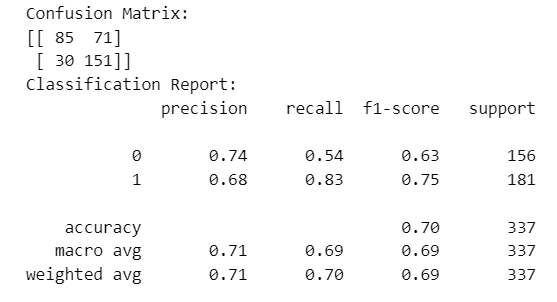
\includegraphics[width=0.6\linewidth]{capture_modele_21.png}
    \caption{Matrice de confusion pour \textit{network\_fev} avec le modèle d'ensemble.}
\end{figure}

\textbf{Interprétation :} La matrice de confusion montre une classification modérée, avec une précision de 0.70 et un F1-score de 0.69 pour \textit{network\_fev}. Le modèle d'ensemble a bien capté la majorité des classes, avec des améliorations légères par rapport aux modèles individuels.

\begin{figure}[H]
    \centering
    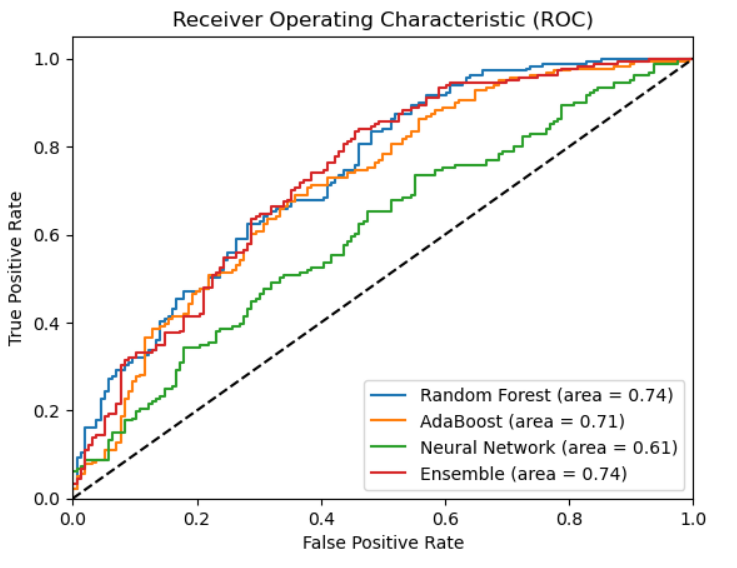
\includegraphics[width=0.7\linewidth]{capture_modele_22.png}
    \caption{Courbe ROC pour \textit{network\_fev} avec le modèle d'ensemble.}
\end{figure}

\textbf{Interprétation :} La courbe ROC montre que l'ensemble des modèles a un AUC de 0.74, similaire à celui du Random Forest. Cela indique que, bien que le modèle d'ensemble ait permis une meilleure combinaison des prédictions, il n'a pas significativement amélioré la capacité globale de discrimination par rapport aux modèles individuels.

\subsubsection{Résultats pour \textit{retail\_juin}}

Les résultats obtenus avec l'approche d'ensemble sur le dataset \textit{retail\_juin} sont les suivants :

\begin{figure}[H]
    \centering
    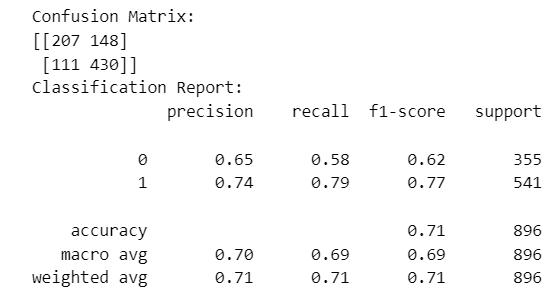
\includegraphics[width=0.6\linewidth]{capture_modele_23.png}
    \caption{Matrice de confusion pour \textit{retail\_juin} avec le modèle d'ensemble.}
\end{figure}

\textbf{Interprétation :} Le modèle d'ensemble a obtenu une précision de 0.71 et un F1-score de 0.71 sur \textit{retail\_juin}, ce qui montre une amélioration par rapport aux modèles de base comme la régression logistique. Cependant, ces résultats restent proches de ceux obtenus par le modèle Random Forest, indiquant que l'ensemble n'a pas significativement surpassé ce dernier.

\begin{figure}[H]
    \centering
    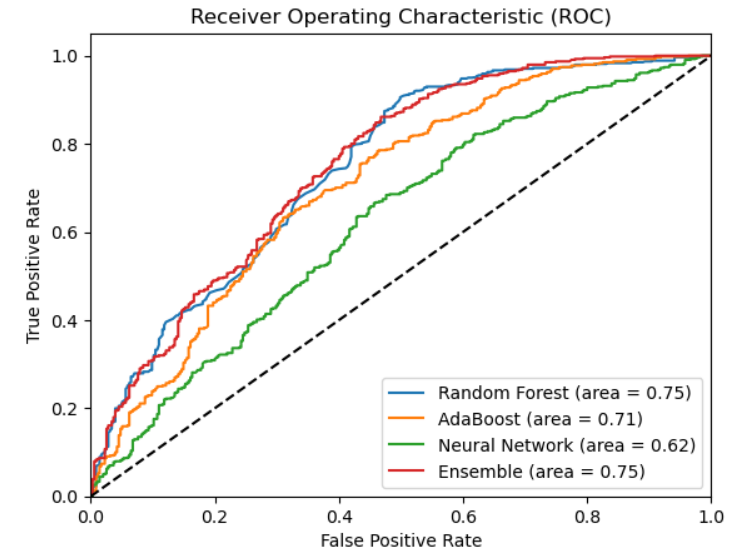
\includegraphics[width=0.7\linewidth]{capture_modele_24.png}
    \caption{Courbe ROC pour \textit{retail\_juin} avec le modèle d'ensemble.}
    \label{fig:roc_juin_ensemble}
\end{figure}

\textbf{Interprétation :} La courbe ROC pour \textit{retail\_juin} montre un AUC de 0.75, similaire au modèle Random Forest. Cela suggère que l'ensemble a capturé efficacement la complexité des données, mais il n'a pas surpassé les performances des modèles individuels.

\subsection{Vérification de surajustement du meilleur modèle}
\subsection{Conclusion}

Dans cette section, on a comparé les performances des modèles de machine learning et de deep learning sur les trois datasets. Les modèles de machine learning, notamment Random Forest, ont bien performé sur les données moins complexes, tandis que les modèles de deep learning, tels que ceux basés sur Keras/TensorFlow, ont mieux généralisé sur des données plus complexes comme \textit{retail\_juin}. L'approche d'ensemble combinant ces deux méthodes n'a apporté que des gains marginaux. En conclusion, le choix du modèle optimal dépend de la complexité des données et du besoin de généralisation.
\section{Vérification du surajustement du meilleur modèle}

Le surajustement (\textit{overfitting}) est un phénomène où un modèle apprend trop spécifiquement les détails et le bruit des données d'entraînement, ce qui lui permet d'obtenir de bonnes performances sur ces données, mais il généralise mal sur des données non vues (jeu de test). Un modèle surajusté aura tendance à surapprendre les particularités des données d'entraînement, au détriment de sa capacité à bien performer sur des données nouvelles.

Pour évaluer si le meilleur modèle présente un phénomène de surajustement, nous avons comparé ses performances sur les jeux de validation et de test. Les résultats présentés ici concernent la data \textbf{network\_may}, et des analyses similaires ont été effectuées pour les autres datasets, où des résultats cohérents ont été obtenus. La figure \ref{fig:overfit} montre ces performances.

\begin{figure}[H]
    \centering
    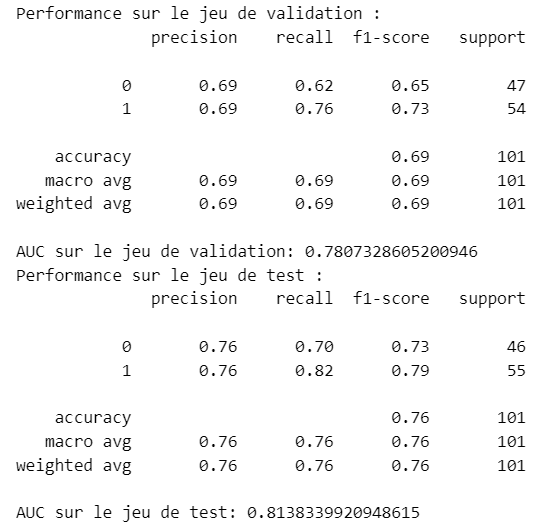
\includegraphics[width=0.6\linewidth]{OVERFIT.png}
    \caption{Performances du modèle sur les jeux de validation et de test pour \textbf{network\_may}}
    \label{fig:overfit}
\end{figure}

\subsection{Analyse des résultats}
Les métriques principales de performance, telles que la précision, le rappel, et le F1-score, ont été calculées sur les jeux de validation et de test. Une AUC (Area Under the ROC Curve) a également été calculée pour évaluer la capacité du modèle à distinguer les classes.

\begin{itemize}
    \item \textbf{Performances sur le jeu de validation :} Le modèle présente une précision et un rappel de 0.69 et 0.76, respectivement, avec un score AUC de \textbf{0.78}. Ces résultats indiquent que le modèle a une capacité modérée à classifier correctement les exemples du jeu de validation.
    \item \textbf{Performances sur le jeu de test :} Les performances sur le jeu de test montrent une légère amélioration, avec une précision et un rappel de 0.76 et 0.82, respectivement, et un score AUC de \textbf{0.81}. Ces résultats sont similaires à ceux du jeu de validation, indiquant que le modèle généralise bien sur des données non vues.
\end{itemize}

\subsection{Conclusion sur le surajustement}
Les performances du modèle sur le jeu de validation et de test sont proches, comme le montre la comparaison des métriques. La différence entre l'AUC sur le jeu de validation (\textbf{0.78}) et l'AUC sur le jeu de test (\textbf{0.81}) est marginale, ce qui suggère que le modèle ne souffre pas de surajustement significatif.

En résumé, le modèle a montré une bonne capacité de généralisation sans surajustement notable, ce qui le rend approprié pour être utilisé sur de nouvelles données. La constance des résultats sur les deux jeux de données reflète la robustesse du modèle.

\section{Profil des Clients Satisfaits et Interprétation des Variables}
\subsection{Résultats pour \textit{network\_fev}}

\textbf{Méthode des Intervalles :}
Les résultats suivants montrent les intervalles de valeurs des variables associées au plus haut niveau de satisfaction des clients. Ces intervalles permettent d'identifier les segments de données qui maximisent la satisfaction client.

\begin{itemize}
    \item L'intervalle le plus satisfaisant pour \textit{activation\_days} correspond à une période allant du **5 août 2015** au **30 juillet 2018**, avec une probabilité de satisfaction de 0.59.
    \item L'intervalle le plus satisfaisant pour \textit{new\_voice\_volume\_moyenne} : [26.40, 32.56], probabilité de satisfaction = 0.62.
    \item L'intervalle pour \textit{new\_data\_amount\_moyenne} : [295.88, 346.13], probabilité de satisfaction = 0.59,etc.
\end{itemize}

La Figure \ref{fig:profil_satisfaction} illustre le profil du client le plus satisfait sur la base de ces intervalles de satisfaction pour le dataset \textit{network\_fev}.

\begin{figure}[H]
    \centering
    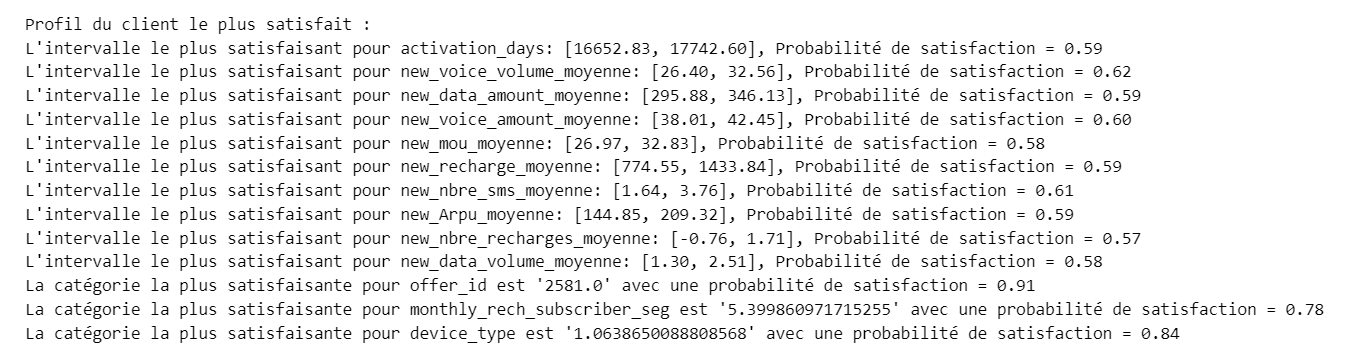
\includegraphics[width=0.9\linewidth]{capture_modele_32.png}
    \caption{Profil du client le plus satisfait pour \textit{network\_fev} basé sur les intervalles de satisfaction.}
    \label{fig:profil_satisfaction}
\end{figure}

\textbf{Méthode d'Interprétation des Effets :}
Cette méthode évalue l'impact d'une augmentation de 10\% des valeurs moyennes des variables sur la probabilité de satisfaction. Voici un résumé des principaux résultats :

\begin{itemize}
    \item Pour \textit{activation\_days}, en augmentant de 10\% la valeur moyenne (du \textbf{22 avril 2015} au \textbf{20 septembre 2017}20 septembre 2017), la probabilité de satisfaction passe de 0.53 à 0.53, soit un changement de 0.50\%.
    \item Pour \textit{new\_voice\_volume\_moyenne}, en augmentant de 10\% la valeur moyenne (de 36.76 à 49.34), la probabilité de satisfaction passe de 0.54 à 0.57, soit un changement de 3.56\%.
    \item Pour \textit{new\_data\_amount\_moyenne}, une augmentation de 10\% fait passer la probabilité de 0.55 à 0.53, soit un changement de -2.22\%, etc.
\end{itemize}

La Figure \ref{fig:interpretation_effets} présente visuellement l'interprétation des effets des variables sur la satisfaction pour \textit{network\_fev}.

\begin{figure}[H]
    \centering
    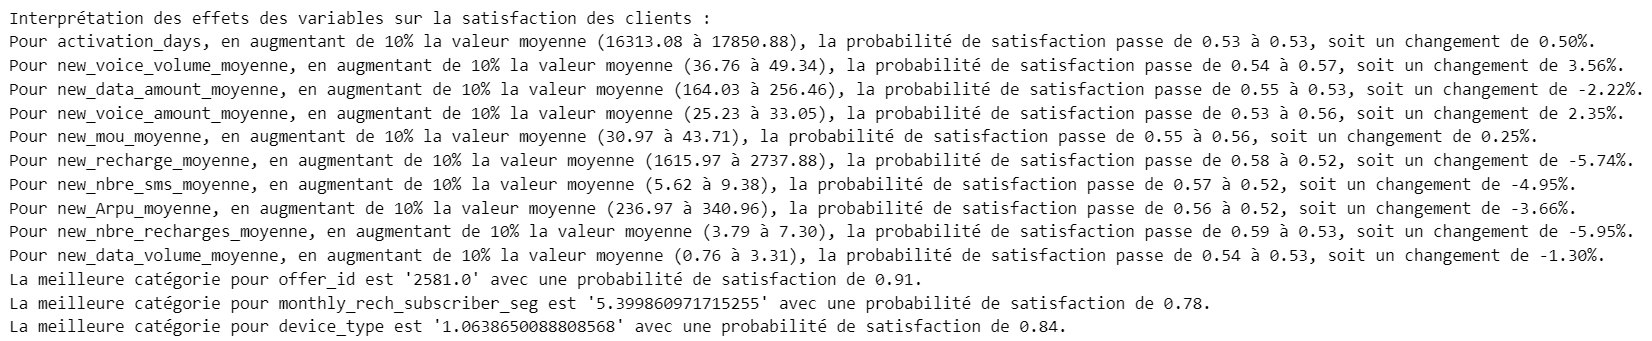
\includegraphics[width=0.9\linewidth]{capture_modele_35.png}
    \caption{Interprétation des effets des variables sur \textit{network\_fev}.}
    \label{fig:interpretation_effets}
\end{figure}

\subsection{Résultats pour \textit{network\_may}}

\textbf{Méthode des Intervalles :}
Les intervalles les plus satisfaisants pour chaque variable incluent :
\begin{itemize}
    \item \textit{Activation Days} : du 3 mars 2021 au 22 septembre 2022, probabilité = 0.69.
    \item \textit{Voice Volume Moyenne} : [17726.43, 24097.83], probabilité = 0.69,etc.
\end{itemize}
La figure \ref{fig:profil_satisfait_may} présente les autres intervalles correspondant aux variables analysées.
\begin{figure}[H]
    \centering
    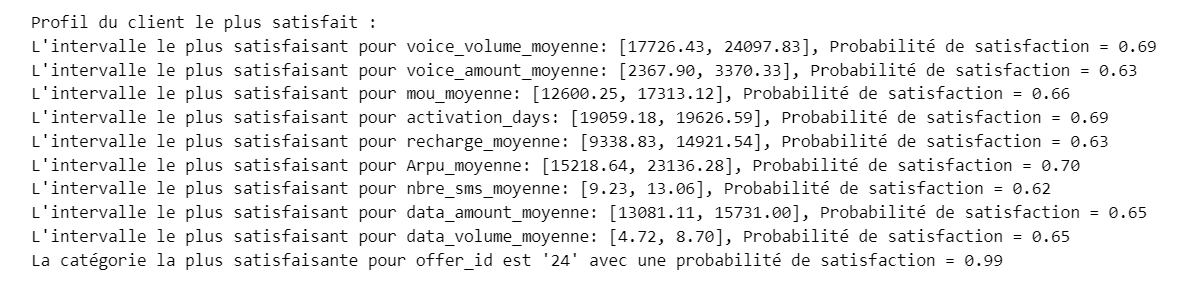
\includegraphics[width=0.9\linewidth]{capture_modele_33.png}
    \caption{Profil du client le plus satisfait pour \textit{network\_may} basé sur les intervalles de satisfaction.}
    \label{fig:profil_satisfait_may}
\end{figure}

\textbf{Méthode d'Interprétation des Effets :}
Quelques exemples d'impact des variables sur la satisfaction :
\begin{itemize}
    \item \textit{Activation Days} : Augmentation de 10\% (du 21 décembre 2016 au 30 août 2019), probabilité de satisfaction passe de 0.54 à 0.66 (+11.63\%).
    \item \textit{Voice Volume Moyenne} : Augmentation de 10\% (3172.58 à 9656.98), probabilité de satisfaction passe de 0.58 à 0.61 (+2.87\%),etc.
\end{itemize}
La figure \ref{fig
} présente également les autres intervalles correspondant aux variables analysées.

\begin{figure}[H]
    \centering
    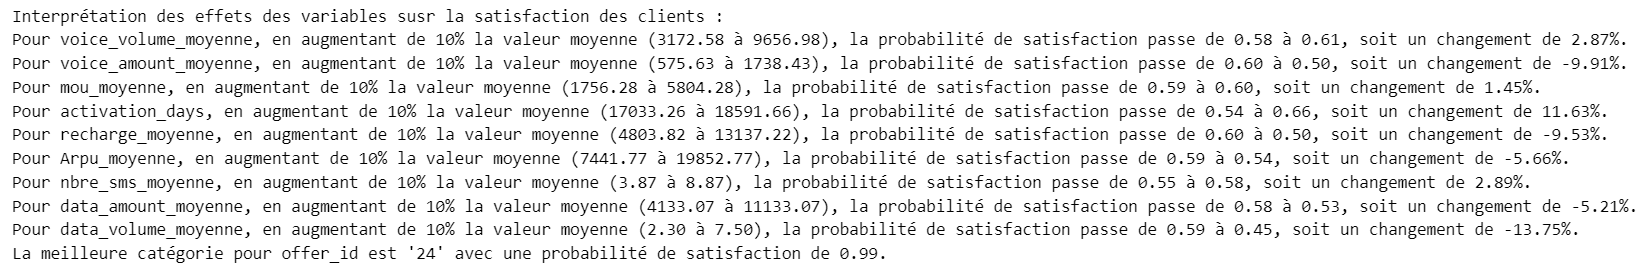
\includegraphics[width=0.9\linewidth]{capture_modele_36.png}
    \caption{Interprétation des effets des variables sur \textit{network\_may}.}
    \label{fig:interpretation_effects_may}
\end{figure}
\subsection{Résultats pour \textit{retail\_juin}}

\textbf{Méthode des Intervalles :}  
Les intervalles les plus satisfaisants pour chaque variable incluent :  
\begin{itemize}
    \item \textit{Activation Days} : du 13 décembre 2016 au 27 mars 2021, probabilité = 0.71.
    \item \textit{Voice Volume Moyenne} : [6470.59, 9894.88], probabilité = 0.66, etc.
\end{itemize}
La figure \ref{fig:profil_satisfait_retail} présente les autres intervalles correspondant aux variables analysées.

\begin{figure}[H]
    \centering
    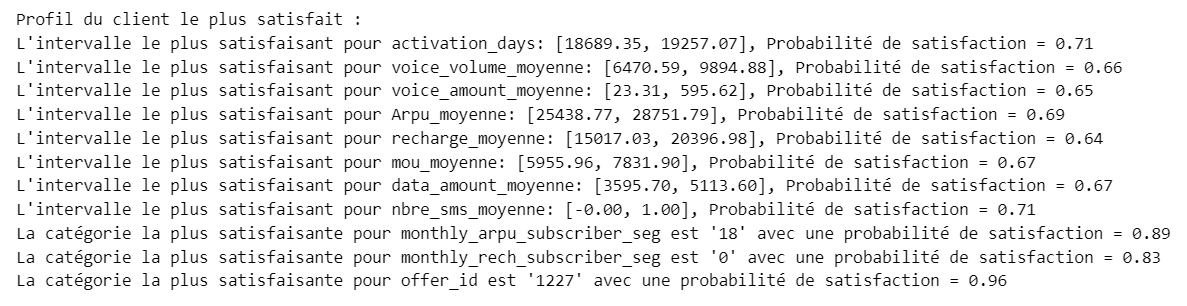
\includegraphics[width=0.9\linewidth]{capture_modele_34.png}
    \caption{Profil du client le plus satisfait pour \textit{retail\_juin} basé sur les intervalles de satisfaction.}
    \label{fig:profil_satisfait_retail}
\end{figure}

\textbf{Méthode d'Interprétation des Effets :}  
Quelques exemples d'impact des variables sur la satisfaction :  
\begin{itemize}
    \item \textit{Activation Days} : Augmentation de 10\% (du 18 juin 2017 au 12 octobre 2020), probabilité de satisfaction passe de 0.55 à 0.56 (+1.33\%).
    \item \textit{Voice Volume Moyenne} : Augmentation de 10\% (1029.51 à 6337.51), probabilité de satisfaction passe de 0.61 à 0.51 (-9.36\%), etc.
\end{itemize}
La figure \ref{fig:interpretation_effects_retail} présente également les autres intervalles correspondant aux variables analysées.

\begin{figure}[H]
    \centering
    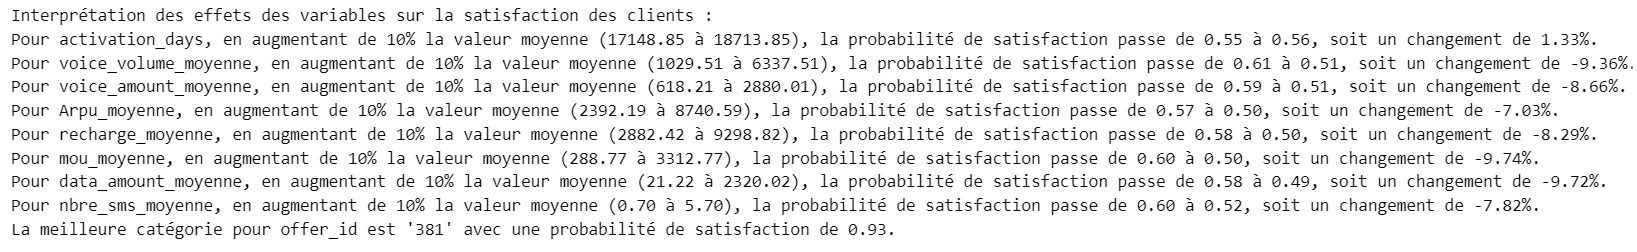
\includegraphics[width=0.9\linewidth]{capture_modele_37.png}
    \caption{Interprétation des effets des variables sur \textit{retail\_juin}.}
    \label{fig:interpretation_effects_retail}
\end{figure}

\subsection{Comparaison des Résultats Entre les Trois Datasets}

Les trois datasets présentent des profils de satisfaction légèrement différents selon les variables analysées.

\begin{itemize}
    \item \textbf{Activation Days :} Le dataset \textit{network\_may} montre l'intervalle le plus récent pour \textit{activation\_days}, tandis que \textit{retail\_juin} couvre une période légèrement plus ancienne. Cependant, les probabilités de satisfaction pour cette variable restent similaires entre les datasets, avec une légère supériorité pour \textit{network\_may}.
    
    \item \textbf{Volume de Voix et de Données :} Pour \textit{network\_fev}, les volumes de voix et de données ont un impact notable sur la satisfaction, avec des probabilités variant entre 0.60 et 0.62. En revanche, ces mêmes variables ont un impact légèrement plus marqué sur \textit{network\_may}, avec des probabilités atteignant 0.66 après variation des valeurs.
    
    \item \textbf{Interprétation des Effets des Variables :} Les résultats d'interprétation montrent que l'augmentation des variables quantitatives, comme \textit{activation\_days} et \textit{new\_Arpu\_moyenne}, entraîne un effet de satisfaction plus fort sur \textit{network\_may}, où des variations de 10\% de ces variables génèrent un changement plus significatif dans la probabilité de satisfaction. À l'inverse, pour \textit{retail\_juin}, les augmentations de 10\% montrent des changements de satisfaction plus modérés.
\end{itemize}

\textbf{Conclusion de la Comparaison :} Les trois datasets révèlent des profils de satisfaction similaires pour certaines variables comme \textit{activation\_days}, mais des différences notables apparaissent pour les volumes de voix et de données, notamment sur \textit{network\_may}. De plus, les effets des augmentations de 10\% dans les variables quantitatives se traduisent par des changements plus importants dans les probabilités de satisfaction pour \textit{network\_may} que pour \textit{retail\_juin} et \textit{network\_fev}. Cela souligne l'importance de chaque dataset dans la détermination des facteurs clés de satisfaction.

\section{Conclusion}

Ce chapitre présente les résultats obtenus à l'aide des modèles de machine learning et de deep learning appliqués aux trois datasets : \textit{network\_fev}, \textit{network\_may}, et \textit{retail\_juin}. Les modèles utilisés incluent la régression logistique, l'arbre de décision, et le Random Forest pour la partie machine learning, ainsi que PyTorch et Keras/TensorFlow pour la partie deep learning. De plus, une approche d'ensemble combinant le Random Forest, AdaBoost et un réseau de neurones a été explorée afin d'améliorer la performance globale de classification. Chaque méthode a été analysée et validée à travers plusieurs métriques de performance, incluant la précision, le F1-score, et l'aire sous la courbe ROC (AUC). Enfin, on a proposé une analyse approfondie du profil des clients les plus satisfaits en nous basant sur les résultats des modèles et en examinant les effets des variables.

Le chapitre est structuré de la manière suivante : tout d'abord, les résultats des modèles de machine learning sont présentés, suivis des résultats des modèles de deep learning. Ensuite, une comparaison globale des deux approches est effectuée avant de présenter les résultats du modèle d'ensemble. Finalement, nous analysons le profil des clients satisfaits en nous basant sur les variables clés identifiées à partir des modèles.
